\documentclass[border=3pt]{standalone}

%Drawing
\usepackage{tikz}

%Tikz Library
\usetikzlibrary{angles, quotes, intersections}

%Notation
\usepackage{physics}
\usepackage{bm}

%Styles
\tikzset{univec/.style={thick, red, -latex}}

\begin{document}
	
	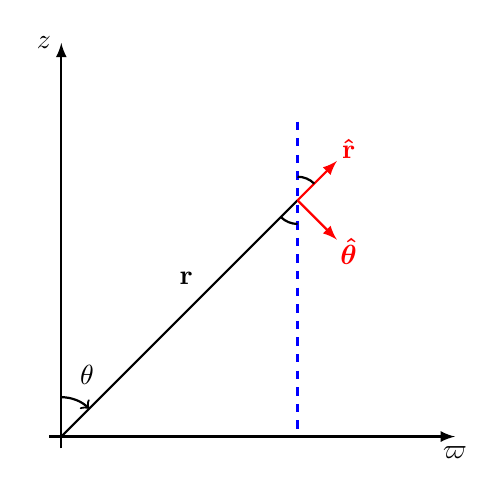
\begin{tikzpicture}
%		%Grid
%		\draw[thin, dotted] (0,0) grid (8,8);
%		\foreach \i in {1,...,8}
%		{
%			\node at (\i,-2ex) {\i};	
%		}
%		\foreach \i in {1,...,8}
%		{
%			\node at (-2ex,\i) {\i};	
%		}
%		\node at (-2ex,-2ex) {0};
		
		%Coordinates
		\coordinate (A) at (3,3);
		\coordinate (B) at (3,4);
		\coordinate (C) at (3,0);
		\coordinate (O) at (0,0);
		\coordinate (D) at (0,5);
		\coordinate (A') at (3.5,3.5);
		
		%Axis
		\draw[thick,-latex] (-1ex,0) -- (5,0) node [below] {$\varpi$};
		\draw[thick,-latex] (0,-1ex) -- (0,5) node [left] {$z$};
		
		%Vectors
		\draw[thick] (O) -- (A) node [pos=0.6, above left] {$\vb{r}$};
		
		%Unit Vectors
		\draw[univec] (A) -- (3.5,3.5) node [pos=1.3] {$\vu{r}$};
		\draw[univec] (A) -- (3.5,2.5) node [pos=1.3] {$\vu*{\theta}$};
		
		%Help Lines
		\draw[thick, dashed, blue] (B) -- (C);
		
		%Angles
		\pic[draw, <-, thick, "$\theta$", angle eccentricity=1.7] {angle = A--O--D};
		\pic[draw, thick, angle radius=0.3cm] {angle = A'--A--B};
		\pic[draw, thick, angle radius=0.3cm] {angle = O--A--C};
		
	\end{tikzpicture}
	
\end{document}